% vim: set textwidth=78 autoindent:
% !TeX root = user_guide.tex

\chapter{Arbeiten mit OGC-Daten}\label{work_ogc}

% when the revision of a chapter has been finalized, 
% comment out the following line:
%\updatedisclaimer

QGIS unterstützt WMS und WFS als Datenquellen. Die WMS-Unterstützung ist nativ,
die WFS-Unterstützung als Plugin integriert.

\section{Was sind OGC-Daten?}\index{OGC!Einführung}

Das Open Geospatial Consortium (OGC)  ist eine internationale Organisation
mit mehr als 300 Mitgliedern aus kommerziellen und behördlichen Bereichen,
aus der Forschung sowie aus Vereinen (Non-Profit). Die Mitglieder entwickeln
und implementieren Standards für den Austausch r�umlicher Daten
(Datendienste), GIS-Datenprocessing und standardisierte Bereitstellung von Geodaten.

Zur Beschreibung von geographischen Objekten in einem einfachen Datenmodell
wurden eine steigende Zahl von Spezifikationen entwickelt, die spezielle
Bedürfnisse der Interoperabilit�t bedienen, räumliche Informationen und GIS
einbezogen. Weitere Informationen können unter
\url{http://www.opengeospatial.org/} abgerufen werden.

Wichtige OGC-Spezifikationen sind:

\begin{itemize}
\item \textbf{WMS} - Web Map Service
\item \textbf{WFS} - Web Feature Service
\item \textbf{WCS} - Web Coverage Service
\item \textbf{CAT} - Web Catalog Service
\item \textbf{SFS} - Simple Features for SQL
\item \textbf{GML} - Geography Markup Language
\end{itemize}

OGC-Dienste werden vermehrt zum Austausch von geographischen Daten zwischen
unterschiedlichen GIS-Systemen und -implementierungen verwendet.
QGIS unterstützt mittlerweile drei der oben genannten Spezifikationen;
einerseits SFS (durch den Postgresql/PostGIS Datenprovider, vgl.
\ref{label_postgis}) sowie als WFS und WMS als Klient.

\section{WMS-Klient}\label{sec:ogc-wms}\index{WMS!Klient}\index{OGC!WMS!Klient}\index{Rasterlayer!WMS}

\subsection{Übersicht über die
WMS-Unterstützung}\label{sec:ogc-wms-about}\index{WMS!Klient!Übersicht}

Derzeit kann QGIS als WMS-Klient eingesetzt werden. Es unterstützt die
Versionen 1.1, 1.1.1 und 1.3 der WMS-Server. Gut getestet wurden die
öffentlich verfügbaren Server wie beispielsweise DEMIS oder NASAs JPL
OnEarth-Server.

WMS-Server liefern Daten aufgrund einer Anfrage eines Klienten (hier QGIS)
als Rasterbild aus. Dabei spielen Ausdehnung, Anzahl der angefragten Layer,
Symbolisierungen und Transparenz eine Rolle. Der WMS-Server holt die
benötigten Daten dann aus seiner Datenquelle hervor, rendert diese in eine
Rasterkarte und sendet das fertige Bild zurück zum Klienten. Das für QGIS
typische Rasterformat ist in aller Regel JPEG oder PNG.

WMS ist ein komplett auf Übertragung ausgelegter Dienst (REST =
Representational State Transfer). Daraus resultiert die Tatsache, dass die
von QGIS generierte URL für das Bild auch in einem Browser eingesetzt werden
kann. Das Resultat dieser Anfrage sieht in der Regel genauso aus wie in QGIS.
Das ist besonders hilfreich, wenn es beim Einsatz von WMS Probleme geben
sollte. Da es sehr viele unterschiedle WMS-Server-Anbieter am Markt gibt (und
alle die WMS-Spezifikation etwas unterschiedlich interpretieren), ist eine
Überprüfung im Browser sehr hilfreich.

WMS-Layer können sehr einfach hinzugefügt werden, solange man die URL des
Servers kennt, eine Verbindung über HTTP zu diesem Server besteht und der
angefragte Server auch HTTP versteht.

\subsection{WMS-Server auswählen}
\label{sec:ogc-wms-servers}\index{WMS!Server!Auswahl}

Wenn Sie die WMS Funktion zum ersten Mal verwenden, sind noch keine Server
definiert, mit denen Sie sich verbinden können. Sie starten die Funktion,
indem Sie auf das Icon \toolbtntwo{mActionAddWmsLayer}{WMS-Layer hinzufügen}
in der Werkzeugleiste klicken oder im Menü
\mainmenuopt{Layer} \arrow \dropmenuopttwo{mActionAddWmsLayer}{WMS-Layer hinzufügen}
auswählen.

Der Dialog \dialog{Layer von einem Server hinzufügen} erscheint dann. Beim
ersten laden eines WMS-Layers sind noch keine Server definiert. Sie können
aber einige vordefinierte Server hinzufügen, indem Sie auf den Knopf
\button{Standard-Server ergänzen} klicken. Dadurch werden mehrere Server
hinzugefügt (z.B. der NASA WMS-Server). Um einen neuen Server selbst zu
definieren klicken Sie auf \button{Neu} und geben dann die Parameter, die zur
Verbindung benötig werden, ein (vgl. Tabelle \ref{tab:wms_connection_parms}):

\begin{table}[h]\index{WMS!Klient!Verbindungsparameter}
\centering
\caption{WMS Verbindungs-Parameter}\label{tab:wms_connection_parms}\medskip
 \begin{tabular}{|l|p{11cm}|}
\hline Name & Ein Name für diese Verbindung. Dieser Name wird in der
Auswahlbox der vorhandenen WMS-Server erscheinen. \\
\hline URL \index{WMS!URL} & Die URL des Servers, der die Daten vorhält.
Dieser Name muss ein auflösbarer Host-Name sein.\\
\hline Benutzername \index{WMS!Authentifizierung} & Benutzername, um auf
einen abgesicherten WMS Server zuzugreifen. Dieser Parameter ist optional. \\
\hline Passwort & Passwort für einen durch Authentifizierung abgesicherten
WMS Server. Dieser Parameter ist optional. \\
\hline
\end{tabular}
\end{table}

Wenn Sie einen Proxy-Server aufsetzen müssen, um WMS-Dienste auf dem
Internet zu empfangen, können Sie die entsprechenden Optionen im Reiter
\tab{Proxy} unter \mainmenuopt{Einstellungen} \arrow
\dropmenuopttwo{mActionOptions}{Optionen} angeben und mit dem
Kontrollkästchen \checkbox{Proxy für Webzugriff benutzen} aktivieren. Wenn
Sie die WMS-Verbindung einmal gesetzt haben, ist sie für zukünftige Sitzungen
gespeichert. Vergewissern Sie sich auch, dass Sie die richtige
Proxyeinstellung aus dem \dropmenuopt{Proxytyp} Menü ausgewählt haben.

\begin{Tip}[h]\caption{\textsc{WMS-Server-URLs}}
Stellen Sie sicher, dass Sie die Basis-URL des Servers eingeben.
Achten Sie darauf, dass keine Fragmente wie \usertext{request=GetCapabilities}
oder \usertext{version=1.0.0} in der URL enthalten sind.\index{WMS!Server!URL}
\end{Tip}

\subsection{Einen WMS-Layer laden}\label{sec:ogc-wms-layers}\index{WMS!Klient!Layer}

Nachdem Sie erfolgreich alle benötigten Parameter eingegeben haben können Sie
den Knopf \button{Verbinden} drücken und die Capabilities des Server holen.
Daraus liest QGIS das unterstützte Bildformat, die verfügbaren Layer, die
Stile sowie die verfügbaren Koordinatenbezugssysteme (KBS).
Da dies eine Netzwerkoperation ist, hängt die Geschwindigkeit der Antwort des
Servers von Ihrer Netzwerkgeschwindigkeit ab. Während die Daten vom Server
heruntergeladen werden, wird der Fortschritt in der linken unteren Ecke des
WMS-Plugin Dialogs angezeigt.

Ihr Bildschirm sollte in etwa so wie der in Abbildung \ref{fig:connection_wms}
aussehen. Dort ist die Antwort des NASA JPL OnEarth WMS-Servers exemplarisch
dargestellt.

\begin{figure}[ht]
  \begin{center}
  	\caption{Dialog zum Hinzufügen eines WMS-Server mit verfügbaren Layern \nixcaption}\label{fig:connection_wms}
	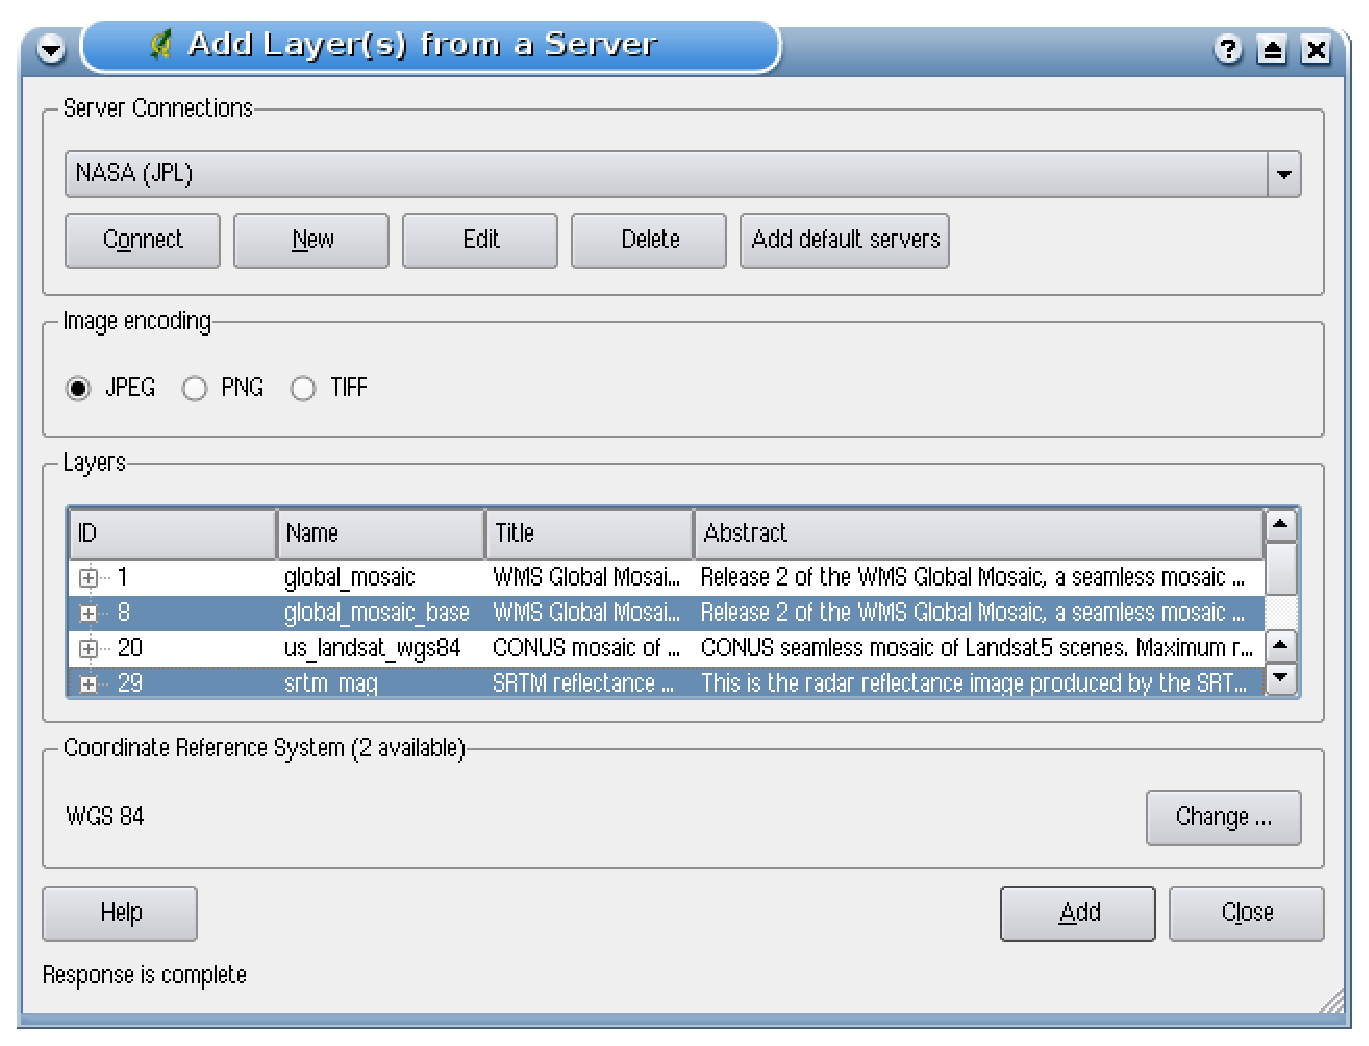
\includegraphics[clip=true,width=15cm]{connection_wms}
  \end{center}
\end{figure}

\minisec{Bildkodierung}

Der Abschnitt über die \guiheading{Bildkodierung} gibt die Bildformate an,
die der Server und QGIS unterstützen. Wählen Sie ein Format aus, das ihren
Ansprüchen entspricht.

\begin{Tip}[h]\caption{\textsc{Bildkodierung}}
In der Regel bieten WMS-Server JPEG oder PNG als Bildkodierung an.
JPEG hat eine bildverschlechternde Kompression, während PNG zumeist die
Qualität der ursprünglichen Rasterdaten widerspiegelt.

Benutzen Sie JPEG wenn Ihre WMS-Daten photographischer Natur
(Luftbilder/Orthophotos) sind und/oder Sie eine geringe qualitative
Beeinträchtigung in der Bildqualität nicht stört.
Verglichen zum PNG reduziert diese kleine Unannehmlichkeit den Datentransfer
bis zum Faktor 5.

Benutzen Sie PNG wenn sie Transparenz und/oder eine exakte Wiedergabe der
Originaldaten benötigen und Sie den erhöhten Datentransfer in Kauf nehmen
können.
\index{WMS!Bildauflösung}
\end{Tip}

\minisec{Optionen}

Der Bereich Optionen im Anfangsdialog bietet ein Textfeld, wo der Name eines 
WMS Layers eingetragen werden kann. Dieser Name wird in der Legende angezeigt, 
nachdem die Layer geladen wurden.

Wenn die OnlineRessource-URL des GetCapabilities-document anders lautet als die 
URL, die in den Verbindunsgparametern vorgegebenen ist, fragt QGIS welche URL 
verwendet werden soll. Entsprechend ihrer Angabe wird QGIS dies dann automatisch 
speichern. Über die Kontrollkästchen \checkbox{GetMap-URL ignorieren} und 
\checkbox{GetFeatureInfo-URL ignorieren} können Sie es selbst festlegen bzw. ändern.  

\minisec{Layer}\label{ogc-wms-layers}

Der Abschnitt der \guiheading{Layer} listet alle verfügbaren Layer des
WMS-Servers auf.
Sie werden bemerkt haben, dass einige Layer aufklappbar sind, was bedeutet,
dass der WMS-Server für diese Layer unterschiedliche Stile bereitstellt.

Sie könnten mehrere Layer auf einmal auswählen, jedoch nur einen Stil pro
Layer. Wenn mehrere Layer ausgewählt wurden, kombiniert der WMS-Server diese
und liefert sie als ein Bild an QGIS.

\begin{Tip}[h]\caption{\textsc{WMS-Layersortierung}}
Über den Reiter Layerreihenfolge können Sie vor dem Laden der 
ausgewählten WMS-Layer eine Reihenfolge festlegen, wie sie in der QGIS Legende 
eingereiht werden sollend, also von oben nach unten.\index{WMS!Server!Layersortierung}
\end{Tip}

\minisec{Transparenz}\label{ogc-wms-transparency}

In der vorliegenden Version von QGIS wird die Transparenz standardmäßig
eingeschaltet, sofern der Server diese unterstützt. Daher existiert keine
separate Option im Dialog. In der Theorie erlaubt dies das Überlagern von
WMS-Layern über andere Layer (Raster, Vektor oder andere WMS-Layer), sodass
man die darunterliegenden Layer noch sehen kann.

\begin{Tip}[h]\caption{\textsc{Transparenz von WMS-Layern}}
Tranzparenz hängt von der verwendeten Bildkodierung ab: PNG und GIF
unterstützen Transparenz, JPEG hingegen nicht. \index{WMS!Transparenz}
\end{Tip}

\minisec{Koordinatensystem}
\index{WMS!KBS}
\index{WMS!Koordinatensystem}
\index{OGC!KBS}
\index{OGC!Koordinatensystem}
\index{Projektion!WMS}
\index{Projektion!KBS}
\index{Projektion!Koordinatensystem}
\index{KBS}
\index{Koordinatenbezugssystem}

Koordinatensystem ist die Bezeichnung des OGC für das
Koordinatenbezugssysteme (KBS).

Jeder WMS-Layer kann in mehreren Koordinatensystemen dargestellt werden;
ausschlaggebend sind die angebotenen System des WMS-Servers.
Sie haben evtl. bemerkt, dass sich diese in der Spaltenüberschrift
basierend auf dem ausgewählten Layer, verändert.

Um ein Koordinatenbeszugsystem auszuwählen, klicken Sie auf den Knopf
\button{Verändere...}. Es öffnet sich ein Fenster ähnlich der Abbildung
\ref{fig:projections} in Abschnitt \ref{label_projstart}. Der einzige
Unterschied ist der, dass dort nur die Koordinatenbezugssysteme angezeigt
werden, die auch vom WMS-Server angeboten werden.

\begin{Tip}[h]\caption{\textsc{WMS-Projektionen}}
Um die besten Resultate zu erreichen, fügen Sie Ihrem Projekt als
erstes die WMS-Layer hinzu. Dadurch stellt QGIS das Koordinatenbezugssysteme
auf die des WMS-Servers ein. Die On-the-fly Projektion funktioniert nur für
Vektorlayer (vgl. Kapitel \ref{sec:projection-specifying}).
Falls Sie einen WMS-Layer später in einem unterschiedlichen Koordinatensystem
hinzufügen, können unvorhersehbare Ereignisse auftreten.
\end{Tip}

\subsection{WMS Serversuche}\label{sec:serversearch}
\index{WMS!Serversuche}
\index{WMS!Suche}
\index{OGC!Suche}

In QGIS ist es möglich, auf Basis von Schlüsselworten nach
WMS Servern im Internet zu suchen. In Abbildung~\ref{fig:searchtab} sehen Sie
den neuen Reiter \tab{Serversuche} im \dialog{WMS-Layer hinzufügen} Dialog.

\begin{figure}[ht]
  \begin{center}
        \caption{Dialog für die Suche von WMS Servern \nixcaption}\label{fig:searchtab}
        \includegraphics[clip=true,width=0.6\textwidth]{wms_server-search}
  \end{center}
\end{figure}

Dazu geben Sie ein Wort nach dem Sie suchen möchten in das Textfeld im
oberen Bereich des Dialogs ein und klicken dann auf den Knopf
\button{Suchen}. Nach einer kurzen Weile werden dann die Ergebnisse
aufgelistet. 

Sie können nun die Ergebnisse durchgehen und wenn Sie einen passenden Server
gefunden haben, wählen Sie diesen mit der linken Maustaste an und klicken
dann auf den Knopf \button{Gewählte Zeile der WMS-Liste hinzufügen}. Dadurch
gelangen Sie automatisch zum Reiter \tab{Server}.

Die Liste der zur Verfügung stehenden WMS Server ist automatisch erweitert
und abgespeichert worden. Um sich mit dem gerade neu ausgewählten WMS Server
zu verbinden, wählen Sie diesen aus der Server Liste aus und klicken dann auf
den Knopf \button{Verbinden}.

Diese Suchfunktion ist ein Frontend zur API von \url{http://geopole.org}.

\subsection{Tilesets}\label{sec:tilesets}
\index{WMS!tileset}
\index{WMS!WMS-C}

Wenn Sie WMS-C (Cached WMS) Dienste, wie \url{http://labs.metacarta.com/wms-c/Basic.py} 
nutzen, können Sie im Reiter \tab{Tilesets} durch die 'Tiles' browsen, die durch den 
Server bereitgestellt werden. Sie sehen dort auch zusätzliche Informationen, wie 
Größe, Format oder das unterstützte KBS (Koordinatenbezugsystem).

In Kombination mit dieser Funktion können Sie im Menü \mainmenuopt{Ansicht} auch 
die \dropmenuopt{Kachelmaßstabsauswahl} öffnen und darüber die vorhanden Maßstäbe 
mittels eines Schiebereglers auswählen und anzeigen. 

\subsection{Das Abfragewerkzeug}\label{sec:ogc-wms-identify}
\index{WMS!Abfragen}
\index{Abfragen!WMS}

Nachdem Sie einen Layer von einem WMS-Server geladen haben, können Sie
die Layer mit dem Werkzeug \toolbtntwo{mActionIdentify}{Objekte Abfragen}
abfragen, sofern der WMS-Server diese Funktion unterstützt. Ein Klick auf
einen Pixel stellt dann eine Abfrage an den WMS-Server für diesen Pixel.
Das Ergebnis wird in Textform geliefert. Die Formatierung hängt von dem
jeweilig verwendeten WMS-Server ab.

\subsection{Eigenschaften}\label{sec:ogc-wms-properties}\index{WMS!Layereigenschaften}\index{Rasterlayer!Layereigenschaften}

Nach erfolgreichem Hinzufügen eines WMS-Layers können Sie die Eigenschaften
des WMS-Servers mit einem Rechtsklick auf den Layernamen in der Legende das
Kontextmenü aufrufen. Der Knopf \button{Eigenschaften} öffnet ein Dialogfenster.

\minisec{Metadaten}\label{sec:ogc-wms-properties-metadata}
\index{Rasterlayer!Metadaten}
\index{WMS!Metadaten}
\index{WMS!Capabilities}

Der Reiter \tab{Metadaten} im Kontextmenü zeigt eine Vielzahl von
Informationen über den WMS-Server. Diese Infos sind dem Capabilities-Dokument
des Servers entnommen.

Viele Definitionen können dem offiziellen Standarddokumenten
\cite{OGCWMS010101web}, \cite{OGCWMS010300web} entnommen werden; hier nur
eine kleine nützliche Auswahl:

\begin{itemize}[label=--]
\item \textbf{Servereigenschaften}
\begin{itemize}[label=--]
\item \textbf{WMS Version}
    - Die WMS-Version, die vom Server unterstützt wird.
\item \textbf{Bildformate}    
    - Eine Liste der MIME-Typen mit denen der Server antworten kann. QGIS
      unterstützt jedes Format, welches die darunterliegende Bibliothek QT
      unterstützt, mindestens aber \texttt{image/png} und \texttt{image/jpeg}.
\item \textbf{Abfrageformate} 
    - Eine Liste der MIME-Typen mit denen der Server auf Pixel-Abfragen
      antworten kann. Derzeit wird von QGIS nur der Typ \texttt{text-plain}
      unterstützt.
\end{itemize}
\item \textbf{Layereigenschaften}
\begin{itemize}[label=--]
\item \textbf{ausgewählt}
    - Gibt an, ob dieser Layer während des Hinzufügens des Server ausgewählt
      war.
\item \textbf{sichtbar}
    - Gibt an, ob der Layer in der Legende angezeigt wird oder nicht. (noch
      nicht verwendet in der aktuellen Version von QGIS).
\item \textbf{Kann abfragen}
    - Gibt an, ob der Layer auf Abfragen Ergebnisse zurückgibt.
\item \textbf{Kann Transparenz}
    - Gibt an, ob der Layer transparent gezeichnet werden kann. Diese Version
      verwendet ein hardcodiertes \textsl{Ja}, sofern die Bildkodierung
      Transparenz bietet.
\item \textbf{Kann reingezoomt werden}
    - Gibt an, ob dieser Layer gezoomt werden kann. Diese Version von QGIS
      verwendet standardmäßig \textsl{Ja}. Daher kann es sein, dass einige
      Layer komisch aussehen, die diese Funktion nicht unterstützen.
\item \textbf{Kaskadierend}
    - WMS-Server könnes als Proxy zwischen anderen WMS-Servern agieren, um
      Rasterdaten für einen Layer anzufordern. Dieser Eintrag gibt an,
      wieviele WMS-Server angefragt werden müssen, um die Daten zu bekommen.
\item \textbf{Fixierte Höhe}
    - Gibt an, ob der Layer eine feste Pixeldimension hat. Diese Version von
      QGIS nimmt an, dass alle WMS-Layer diesen Wert nicht gesetzt haben.
      Daher kann es sein, dass einige Layer komisch aussehen, die diese
      Funktion nicht unterstützen.
\item \textbf{WGS 84 Boundingbox}
    - Gibt die Boundingbox eines Layers in WGS84-Koordinaten an. Einige
      WMS-Server setzen diese Werte nicht korrekt (z.B. stehen darin manchmal
      UTM-Koordinaten), sodass bei solchen Layern in QGIS der Eindruck
      entsteht, sehr weit herausgezoomt zu sein. Der Webmaster des
      WMS-Servers sollte dann auf dieses Problem aufmerksam gemacht werden.
      Das WMS XML-Element ist \texttt{LatLonBoundingBox},
      \texttt{EX\_GeographicBoundingBox} oder die CRS:84 \texttt{BoundingBox}.
\item \textbf{verfügbare Koordinatensysteme} 
    - Die Projektionen, in denen dieser Layer dargestellt werden kann. Diese
      sind dem Capabilities-Dokument des Servers entnommen.
\item \textbf{verfügbare Stile} 
    - Die Bildstile, in denen dieser Layer dargestellt werden kann.
\end{itemize}
\end{itemize}

\subsection{Einschränkungen des WMS-Klienten}
\label{sec:ogc-wms-limits}\index{WMS!Klient!Einschränkungen}

Nicht alle spezifizierten und möglichen WMS-Klientfunktionalitäten wurden in
diese Version von QGIS implementiert. Einige nennenswerte Ausnahmen seien
kurz erläutert:

\minisec{WMS-Layereigenschaften ändern}
\index{WMS!Layereigenschaften!editieren}

Wenn der Layer über den Knopf \toolbtntwo{mActionAddWmsLayer}{WMS-Layer
hinzufügen} geladen wurde, besteht im Nachhinein keine Möglichkeit, diese
nocheinmal zu ändern.

Als Workaround sollte der Layer komplett gelöscht und mit den gewünschten
Einstellungen erneut vom Server geladen werden.

\minisec{WMS-Server, die eine Authentifizierung benötigen}
\index{WMS!Server!Authentifizierung}
\index{WMS!Server!Einfache Authentifizierung}

Derzeit sind öffentlich zugängliche und abgesicherte WMS Server nutzbar. Ein
abgesicherter WMS Server kann über eine einfache, öffentliche Authentifizierung
eingebunden werden. Sie können die notwendigen (optionalen) Angaben machen,
wenn Sie einen WMS Server hinzufügen, wie in
Kapitel~\ref{sec:ogc-wms-servers} beschrieben.

\begin{Tip}[ht]\caption{\textsc{Zugriff auf abgesicherte OGC-Layer}}
Wenn Sie Zugriff auf OGC-Layer benötigen, die anders als durch
einfache, öffentliche Authentifizierung abgesichert sind, können Sie
InteProxy als transparenten Proxy verwenden. Dieser unterstützt verschiedene
Methoden der Authentifizierung. Weitere Informationen zu diesem Thema finden
Sie auf der Webseite \url{http://inteproxy.wald.intevation.org}.
\index{WMS!abgesicherter Layer!}\index{OGC!Authentifizierung}
\end{Tip}

%
% WMS-server
%

%%FIXME
\section{WMS Server}\label{sec:ogc-wmsserver}
\index{WMS!server}

QGIS mapserver is an open source WMS 1.3 implementation which, in addition,
implements advanced cartographic features for thematic mapping. The QGIS
mapserver is a FastCGI/CGI (Common Gateway Interface) application written in
C++ that works together with a webserver (e.g. Apache, Lighttpd). 


It uses QGIS as backend for the GIS logic and for map rendering. Furthermore the 
Qt library is used for graphics and for platform independent 
C++ programming. In contrast to other WMS software, the QGIS mapserver uses 
cartographic rules in SLD/SE as a configuration language, both for the server 
configuration and for the user-defined cartographic rules. 

Moreover, the QGIS mapserver project provides the “Publish to Web” plugin, a 
plugin for QGIS desktop which exports the current layers and symbology as a 
web project for QGIS mapserver (containing cartographic visualisation rules 
expressed in SLD).

As QGIS desktop and QGIS mapserver use the same visualization libraries, the
maps that are published on the web look the same as in desktop GIS. The 
Publish to Web plugin currently supports basic symbolization, with more complex 
cartographic visualisation rules introduced manually. As the configuration is 
performed with the SLD standard and its documented extensions, there is only 
one standardised language to learn, which greatly simplifies the complexity 
of creating maps for the Web.

Further information is available at: \\
\url{http://karlinapp.ethz.ch/qgis\_wms/} \\
\url{http://www.qgis.org/wiki/QGIS\_mapserver\_tutorial} \\
\url{http://linfiniti.com/2010/08/qgis-mapserver-a-wms-server-for-the-masses/}


\section{WFS und WFS-T Klient}\label{sec:ogc-wfs}

In QGIS verhält sich ein WFS-Layer weitestgehend wie ein anderer Vektorlayer.
Sie können Objekte abfragen, auswählen und sich die Attributtabelle
anschauen. Das WFS-Plugin unterstützt als WFS-T auch das Editieren von
WFS-Layern. Um das WFS Plugin zu starten öffnen Sie das Menü 
\mainmenuopt{Plugins} \arrow \dropmenuopttwo{mActionShowPluginManager}{Plugins
verwalten}, aktivieren Sie das Kontrollkästchen \checkbox{WFS-Plugin} und
drücken Sie dann auf \button{OK}.

In der Werkzeugleiste erscheint nun das
\toolbtntwo{mIconAddWfsLayer}{WFS-Layer hinzufügen} Icon, mit dem Sie den
Dialog \dialog{WFS-Layer von Server hinzufügen} öffnen können. Das Hinzufügen
eines WFS-Layers ist fast identisch mit dem Vorgehen beim Laden eines
WMS-Layers. Der aktuelle Unterschied ist, dass keine Beispielserver
vordefiniert sind, daher soll dies in dem folgenden Beispiel vorgeführt
werden.

\subsection{Einen WFS-Layer laden}

In diesem Beispiel verwenden wir den WFS-Server der Firma DMSolution und
laden einen
Layer. Die URL ist:
\begin{verbatim}
http://www2.dmsolutions.ca/cgi-bin/mswfs_gmap
\end{verbatim}

\begin{enumerate}
  \item Laden Sie das WFS-Plugin, falls dies noch nicht geschehen ist. Öffnen
Sie ansonsten den Plugin-Manager und laden Sie es
  \item Klicken Sie auf \toolbtntwo{mIconAddWfsLayer}{WFS-Layer hinzufügen} in der
Werkzeugleiste
  \item Klicken Sie auf \button{Neu}
  \item Tragen Sie \inputtext{Name}{DM Solutions} als Name ein
  \item Tragen Sie die URL ein (siehe oben)
  \item Klicken Sie auf \button{OK}
  \item Wählen Sie ``DM Solutions'' aus dem Menü der vorhandenen Server
  \item Klicken Sie auf \button{Verbinden}
  \item Warten Sie auf die Liste vorhandener Layer des Servers
  \item Klicken Sie auf den Layer \clicklistitem{Parks}
  \item Klicken Sie auf \button{Hinzufügen} um den Layer anzuzeigen
  \item Warten Sie, dass die Daten heruntergeladen und angezeigt werden
\end{enumerate}

Beachten Sie, dass das WFS Plugin auch die Proxyeinstellungen verwendet, die
Sie als Option definiert haben.

\begin{figure}[ht]
  \begin{center}
  	\caption{WFS-Layer hinzufügen \nixcaption}\label{fig:wfs_dmsolutions}
	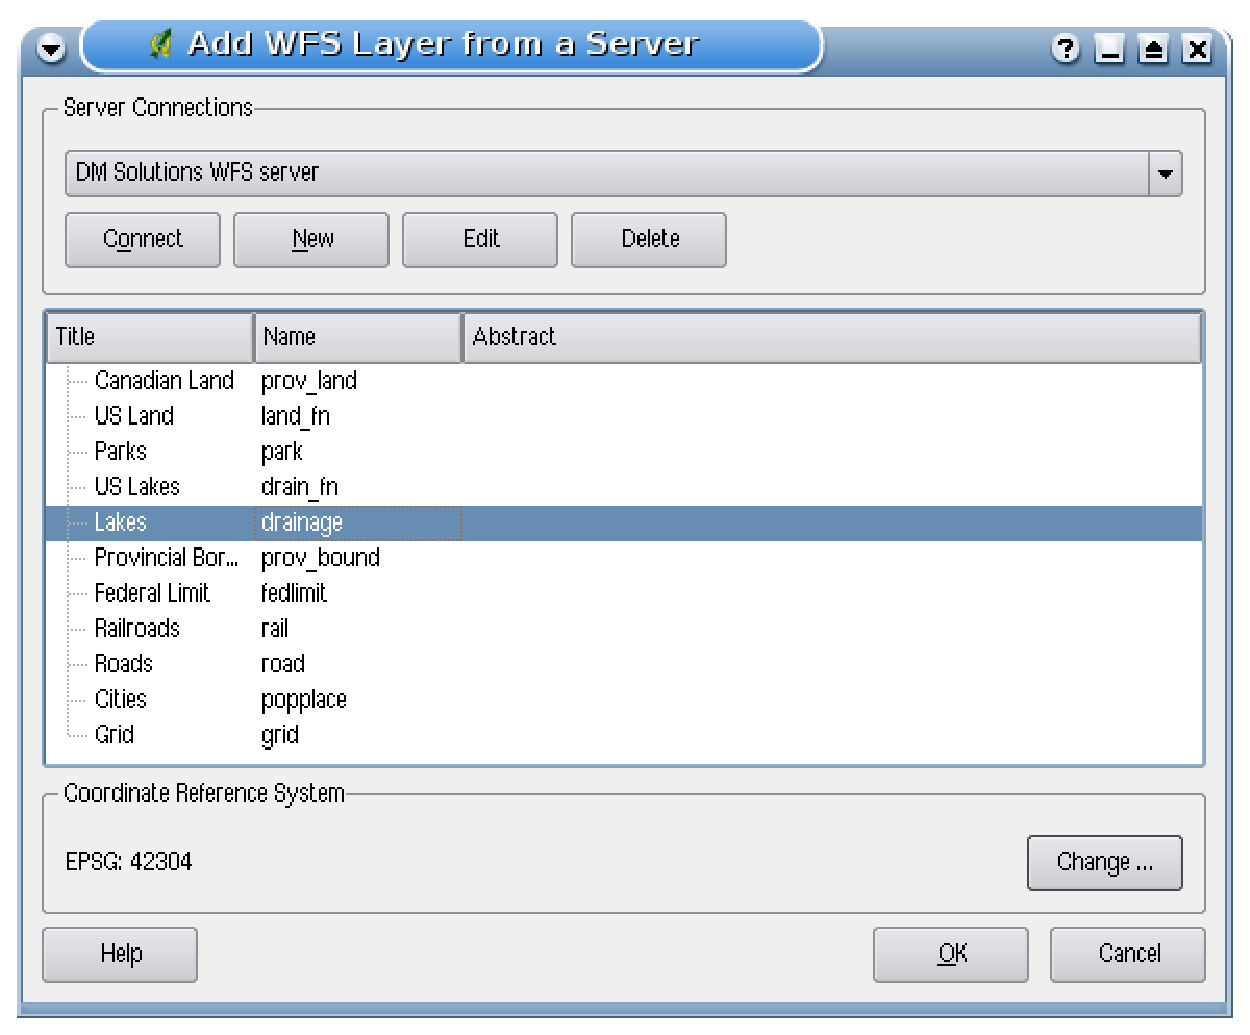
\includegraphics[clip=true,width=0.7\textwidth]{connection_wfs}
  \end{center}
\end{figure}

Wenn Sie das Kontrollkästchen \checkbox{Nur Objekte, die den aktuellen Ausschnitt 
schneiden, laden} nicht aktivieren, werden alle Objekte des Layers geladen. Wenn 
Sie nur einen kleinen Ausschnitt anzeigen wollen, zoomen Sie in den Bereich, 
aktivieren Sie das Kontrollkästchen und stellen eine erneute Anfrage an den 
WFS-Server. Dadurch wird ein BBOX-Parameter mit der aktuellen Ausdehung des 
Kartenfensters hinzugefügt. Dies ist sehr angenehm, wenn Sie nur wenige Objekte 
aus einer sehr großen Karte anzeigen lassen möchten. 

Sie werden sehen, dass der Fortschritt des Herunterladens in der unteren,
linken Ecke des QGIS-Hauptfensters angezeigt wird. Wenn der Layer geladen und
angezeigt wird, können Sie die Objekte auswählen und sich die dazugehörigen
Attributtabellen anzeigen lassen.

Bedenken Sie, dass dieses Plugin am besten mit WFS Servern unter UMN
MapServer funktioniert und dass es noch experimentell ist und Fehler auftreten
können, genauso wie Abstürze.

Der Grund hierfür liegt darin, dass aktuell nur WFS 1.0.0 unterstützt wird.
Außerdem wurde bis zu diesem Zeitpunkt noch nicht sehr umfangreich die
Anbindung mit anderen WFS Servern getestet. Wenn Sie Probleme feststellen,
zögern Sie bitte nicht, eine Email an das QGIS Projekt zu schicken oder einen
Fehlerreport zu schreiben. Sie finden eine Liste möglicher Kontakte in
Kapitel~\ref{label_helpsupport}.

\begin{Tip}[h]\caption{\textsc{WFS Server finden}}
Sie können weitere WFS Server mit Hilfe von Google oder
ihrer bevorzugten Suchmaschine finden. Es gibt eine Vielzahl von Listen im
Internet, die Links zu öffentlichen Servern bereitstellen.
\index{WFS!Server!}
\index{WFS!Serversuche!}
\end{Tip}

\begin{Tip}[ht]\caption{\textsc{Abgesicherte WFS Server einbinden}}
Im Dialog \dialog{WFS-Layer hinzufügen} ist es zwar möglich, einen
Benutzernamen und ein Passwort anzugeben. Im Gegensatz zu WMS Servern, ist es
aber momentan noch nicht möglich, auf WFS Server mit einfacher, öffentlicher
Authentifizierung zuzugreifen. Dieses soll in einer der folgenden QGIS
Versionen erfolgen. Bis dahin könnten Sie z.B. InteProxy 
(\url{http://inteproxy.wald.intevation.org}) für die Authentifizierung
verwenden.
\index{WFS!einfache Authentifizierung!}
\index{WFS!abgesicherte WFS server!}
\end{Tip}

\FloatBarrier

